% !TeX spellcheck = en_GB
%%%%%%%%%%%%%%%%%%%%%%%%%%%%%%%%%%%%%%%%%%
%                                        %
%    Engineer thesis LaTeX template      %
%  compliant with the SZJK regulations   %
%                                        %
%%%%%%%%%%%%%%%%%%%%%%%%%%%%%%%%%%%%%%%%%%
%                                        %
%  (c) Krzysztof Simiński, 2018-2022     %
%                                        %
%%%%%%%%%%%%%%%%%%%%%%%%%%%%%%%%%%%%%%%%%%
%                                        %
% The latest version of the templates is %
% available at                           %
% github.com/ksiminski/polsl-aei-theses  %
%                                        %
%%%%%%%%%%%%%%%%%%%%%%%%%%%%%%%%%%%%%%%%%%
%
%
% This LaTeX project formats the final thesis
% with compliance to the SZJK regulations.
% Please to not change formatting (fonts, margins,
% bolds, italics, etc).
%
% You can compile the project in several ways.
%
% 1. pdfLaTeX compilation
%
% pdflatex main
% bibtex   main
% pdflatex main
% pdflatex main
%
%
% 2. XeLaTeX compilation
%
% Compilation with the XeLaTeX engine inserts Calibri font
% in the title page. Of course the font has to be installed.
%

% xelatex main
% bibtex  main
% xelatex main
% xelatex main
%
%
%%%%%%%%%%%%%%%%%%%%%%%%%%%%%%%%%%%%%%%%%%%%%%%%%%%%%%%%%%%%%%
% If you have any questions, remarks, just send me an email: %
%            krzysztof.siminski(at)polsl.pl               %
%%%%%%%%%%%%%%%%%%%%%%%%%%%%%%%%%%%%%%%%%%%%%%%%%%%%%%%%%%%%%%

% We would like to improve the LaTeX templates
% of final theses. By answering the questions
% in the survey whose address your can find below
% you help us to do so. The survey is completely
% anonimous. Thank you!
%
% https://docs.google.com/forms/d/e/1FAIpQLScyllVxNKzKFHfILDfdbwC-jvT8YL0RSTFs-s27UGw9CKn-fQ/viewform?usp=sf_link
%
%%%%%%%%%%%%%%%%%%%%%%%%%%%%%%%%%%%%%%%%%%%%%%%%%%%%%%%%%%%%%%%%%%%%%%%%%

%%%%%%%%%%%%%%%%%%%%%%%%%%%%%%%%%%%%%%%%%%%%%%%
%                                             %
% CUSTOMISATION OF THE THESIS                 %
%                                             %
%%%%%%%%%%%%%%%%%%%%%%%%%%%%%%%%%%%%%%%%%%%%%%%

% Please customise your thesis with the macros below.

% TODO
\newcommand{\Firstnames}{Daniel Bartosz}
\newcommand{\Surname}{Marek}
\newcommand{\Supervisor}{Jakub Nalepa, PhD, DSc}  % supervisor (remove $\langle$ and $\rangle)
\newcommand{\Title}{Extraterrestrial rock segmentation using machine learning}
\newcommand{\TitleAlt}{Segmentacja skał pozaziemskich z wykorzystaniem uczenia maszynowego}
\newcommand{\Program}{Informatics}
\newcommand{\Specialisation}{Computer Graphics and Software}
\newcommand{\Id}{290763} %  (remove $\langle$ and $\rangle)
\newcommand{\Departament}{Department of Algorithmics and Software } % your supervisor's departament  (remove $\langle$ and $\rangle)


% If you have a consultant for your thesis, put their name below ...
% \newcommand{\Consultant}{title first name surname}  %  (remove $\langle$ and $\rangle)
% ... else leave the braces empty:
\newcommand{\consultant}{} % no consultant

% end of thesis customisation
%%%%%%%%%%%%%%%%%%%%%%%%%%%%%%%%%%%%%%%%%%

%%%%%%%%%%%%%%%%%%%%%%%%%%%%%%%%%%%%%%%%%%%%%%%
%                                             %
% END OF CUSTOMISATION                        %
%                                             %
%%%%%%%%%%%%%%%%%%%%%%%%%%%%%%%%%%%%%%%%%%%%%%%

%%%%%%%%%%%%%%%%%%%%%%%%%%%%%%%%%%%%%%%%


%%%%%%%%%%%%%%%%%%%%%%%%%%%%%%%%%%%%%%%%%%%%%%%
%                                             %
%   PLEASE DO NOT MODIFY THE SETTINGS BELOW!  %
%                                             %
%%%%%%%%%%%%%%%%%%%%%%%%%%%%%%%%%%%%%%%%%%%%%%%



\documentclass[a4paper,twoside,12pt]{book}
\usepackage[utf8]{inputenc}
\usepackage[T1]{fontenc}
\usepackage{amsmath,amsfonts,amssymb,amsthm}
\usepackage[polish,british]{babel}
\usepackage{indentfirst}



\usepackage{ifxetex}

\ifxetex
	\usepackage{fontspec}
	\defaultfontfeatures{Mapping=tex—text} % to support TeX conventions like ``——-''
	\usepackage{xunicode} % Unicode support for LaTeX character names (accents, European chars, etc)
	\usepackage{xltxtra} % Extra customizations for XeLaTeX
\else
	\usepackage{lmodern}
\fi



\usepackage[margin=2.5cm]{geometry}
\usepackage{graphicx}
\usepackage{hyperref}
\usepackage{booktabs}
\usepackage{tikz}
\usepackage{pgfplots}
\usepackage{mathtools}
\usepackage{geometry}
\usepackage{subcaption}   % subfigures
\usepackage[page]{appendix} % toc,




\usepackage{csquotes}
\usepackage[natbib=true,backend=bibtex,maxbibnames=99]{biblatex}  % compilation of bibliography with BibTeX
%\usepackage[natbib=true,backend=biber,maxbibnames=99]{biblatex}  % compilation of bibliography with Biber
\bibliography{biblio}

\usepackage{ifmtarg}   % empty commands

\usepackage{setspace}
\onehalfspacing


\frenchspacing



%%%% TODO LIST GENERATOR %%%%%%%%%

\usepackage{color}
\definecolor{brickred}      {cmyk}{0   , 0.89, 0.94, 0.28}

\makeatletter \newcommand \kslistofremarks{\section*{Remarks} \@starttoc{rks}}
  \newcommand\l@uwagas[2]
    {\par\noindent \textbf{#2:} %\parbox{10cm}
{#1}\par} \makeatother


\newcommand{\ksremark}[1]{%
{%\marginpar{\textdbend}
{\color{brickred}{[#1]}}}%
\addcontentsline{rks}{uwagas}{\protect{#1}}%
}










%%%%%%%%%%%%%% END OF TODO LIST GENERATOR %%%%%%%%%%%

%%%%%%%%%%%% FANCY HEADERS %%%%%%%%%%%%%%%
% no capitalisation of headers
\usepackage{fancyhdr}
\pagestyle{fancy}
\fancyhf{}
\fancyhead[LO]{\nouppercase{\it\rightmark}}
\fancyhead[RE]{\nouppercase{\it\leftmark}}
\fancyhead[LE,RO]{\it\thepage}


\fancypagestyle{onlyPageNumbers}{%
   \fancyhf{}
   \fancyhead[LE,RO]{\it\thepage}
}

\fancypagestyle{noNumbers}{%
   \fancyhf{}
   \fancyhead[LE,RO]{}
}


\fancypagestyle{PageNumbersChapterTitles}{%
   \fancyhf{}
   \fancyhead[LO]{\nouppercase{\Firstnames\ \Surname}}
   \fancyhead[RE]{\nouppercase{\leftmark}}
   \fancyfoot[CE, CO]{\thepage}
}




%%%%%%%%%%%%%%%%%%%%%%%%%%%







\newcounter{pagesWithoutNumbers}

%%%%%%%%%%%%%%%%%%%%%%%%%%%
\usepackage{xstring}
\usepackage{ifthen}
\newcommand{\printOpiekun}[1]{%

    \StrLen{\Consultant}[\mystringlen]
    \ifthenelse{\mystringlen > 0}%
    {%
       {\large{\bfseries CONSULTANT}\par}

       {\large{\bfseries \Consultant}\par}
    }%
    {}
}
%
%%%%%%%%%%%%%%%%%%%%%%%%%%%%%%%%%%%%%%%%%%%%%%

% Please do not modify the lines below!
\author{\Firstnames\ \Surname}
\newcommand{\Author}{\Firstnames\ \MakeUppercase{\Surname}}
\newcommand{\Type}{FINAL PROJECT}
\newcommand{\Faculty}{Faculty of Automatic Control, Electronics and Computer Science}
\newcommand{\Polsl}{Silesian University of Technology}
\newcommand{\Logo}{politechnika_sl_logo_bw_pion_en.pdf}
\newcommand{\LeftId}{Student identification number}
\newcommand{\LeftProgram}{Programme}
\newcommand{\LeftSpecialisation}{Specialisation}
\newcommand{\LeftSUPERVISOR}{SUPERVISOR}
\newcommand{\LeftDEPARTMENT}{DEPARTMENT}
%%%%%%%%%%%%%%%%%%%%%%%%%%%%%%%%%%%%%%%%%%%%%%

%%%%%%%%%%%%%%%%%%%%%%%%%%%%%%%%%%%%%%%%%%%%%%%
%                                             %
% END OF SETTINGS                             %
%                                             %
%%%%%%%%%%%%%%%%%%%%%%%%%%%%%%%%%%%%%%%%%%%%%%%




%%%%%%%%%%%%%%%%%%%%%%%%%%%%%%%%%%%%%%%%%%%%%%%
%                                             %
% MY PACKAGES, SETTINGS ETC.                  %
%                                             %
%%%%%%%%%%%%%%%%%%%%%%%%%%%%%%%%%%%%%%%%%%%%%%%

% Put your packages, macros, setting here.



%%%%%%%%%%%%%%%%%%%%%%%%%%%%%%%%%%%%%%%%%%%%%%%%%%%%%%%%%%%%%%%%%%%%%
% listings
% packages: listings or minted
% % % % % % % % % % % % % % % % % % % % % % % % % % % % % % % % % % %

% package listings
\usepackage{listings}
\lstset{%
morekeywords={string,exception,std,vector},% add the keyword you need
language=C++,% C, Matlab, Python, SQL, TeX, XML, bash, ... – vide https://www.ctan.org/pkg/listings
commentstyle=\textit,%
identifierstyle=\textsf,%
keywordstyle=\sffamily\bfseries, %\texttt, %
%captionpos=b,%
tabsize=3,%
frame=lines,%
numbers=left,%
numberstyle=\tiny,%
numbersep=5pt,%
breaklines=true,%
%morekeywords={descriptor_gaussian,descriptor,partition,fcm_possibilistic,dataset,my_exception,exception,std,vector},%
escapeinside={@*}{*@},%
}

% % % % % % % % % % % % % % % % % % % % % % % % % % % % % % % % % % %
% package minted
% \usepackage{minted}

% This package requires a special command line option in compilation
% pdflatex -shell-escape main.tex
% xelatex  -shell-escape main.tex

%%%%%%%%%%%%%%%%%%%%%%%%%%%%%%%%%%%%%%%%%%%%%%%%%%%%%%%%%%%%%%%%%%%%%



%%%%%%%%%%%%%%%%%%%%%%%%%%%%%%%%%%%%%%%%%%%%%%%
%                                             %
% END OF MY PACKAGES, SETTINGS ETC.           %
%                                             %
%%%%%%%%%%%%%%%%%%%%%%%%%%%%%%%%%%%%%%%%%%%%%%%



%%%%%%%%%%%%%%%%%%%%%%%%%%%%%%%%%%%%%%%%


\begin{document}
%\kslistofremarks


%%%%%%%%%%%%%%%%%%%%%%%%%%%%%%%%%%%%%%%%%%%%%%%
%                                             %
%    PLEASE DO NOT MODIFY THE TITLE PAGE!     %
%                                             %
%%%%%%%%%%%%%%%%%%%%%%%%%%%%%%%%%%%%%%%%%%%%%%%


%%%%%%%%%%%%%%%%%%  TITLE PAGE %%%%%%%%%%%%%%%%%%%
\pagestyle{empty}
{
	\newgeometry{top=1.5cm,%
	             bottom=2.5cm,%
	             left=3cm,
	             right=2.5cm}

	\ifxetex
	  \begingroup
	  \setsansfont{Calibri}

	\fi
	 \sffamily
	\begin{center}
	\includegraphics[width=50mm]{\Logo}


	{\Large\bfseries\Type\par}

	\vfill  \vfill

	{\large\Title\par}

	\vfill

	{\large\bfseries\Author\par}

	{\normalsize\bfseries \LeftId: \Id}

	\vfill

	{\large{\bfseries \LeftProgram:} \Program\par}

	{\large{\bfseries \LeftSpecialisation:} \Specialisation\par}

	\vfill  \vfill 	\vfill 	\vfill 	\vfill 	\vfill 	\vfill

	{\large{\bfseries \LeftSUPERVISOR}\par}

	{\large{\bfseries \Supervisor}\par}

	{\large{\bfseries \Departament}\par}

	{\large{\bfseries \Faculty}\par}

	\vfill  \vfill


    % \printOpiekun{\Consultant}

	\vfill  \vfill

    {\large\bfseries  Gliwice \the\year}

   \end{center}
       \ifxetex
       	  \endgroup
       \fi
	\restoregeometry
}



\cleardoublepage

\rmfamily\normalfont
\pagestyle{empty}


%%% Let's start the thesis %%%%

% TODO
\subsubsection*{Thesis title}
\Title

\subsubsection*{Abstract}
(Thesis abstract – to be copied into an appropriate field during an electronic submission – in English.)

\subsubsection*{Key words}
(2-5 keywords, separated by commas)

\subsubsection*{Tytuł pracy}
\begin{otherlanguage}{polish}
\TitleAlt
\end{otherlanguage}

\subsubsection*{Streszczenie}
\begin{otherlanguage}{polish}
(Streszczenie pracy – odpowiednie pole w systemie APD powinno zawierać kopię tego streszczenia.)
\end{otherlanguage}

\subsubsection*{Słowa kluczowe}
\begin{otherlanguage}{polish}
(2-5 slow (fraz) kluczowych, oddzielonych przecinkami)
\end{otherlanguage}




%%%%%%%%%%%%%%%%%% Table of contents %%%%%%%%%%%%%%%%%%%%%%
%\pagenumbering{Roman}
\thispagestyle{empty}
\tableofcontents
\thispagestyle{empty}

%%%%%%%%%%%%%%%%%%%%%%%%%%%%%%%%%%%%%%%%%%%%%%%%%%%%%
\setcounter{pagesWithoutNumbers}{\value{page}}
\mainmatter
\pagestyle{empty}

\cleardoublepage

\pagestyle{PageNumbersChapterTitles}

%%%%%%%%%%%%%% body of the thesis %%%%%%%%%%%%%%%%%

% TODO
\chapter{Introduction}
\label{sec:chapter1}
In 1969, during the Apollo 11 mission, humanity reached the Moon for the first time in history. This phenomenal achievement was possible thanks to countless hours of hard work put in by the brightest engineers and scientists of that time. It was proven possible to reach a new world. The last time humans stood on the Moon was during the Apollo 17 mission in 1972. Since the end of the space race, many uncrewed missions have studied the core and surface of the silver globe. In 2017, the United States National Aeronautics and Space Administration launched a new Moon exploration program. This program aims to reestablish a human presence on the Moon, with the long-term goal of creating a permanent base camp and facilitating human missions to Mars \cite{smith2020artemis}.

Establishing a human presence on another world is challenging due to cosmic radiation, lack of breathable air, high temperature fluctuations and other environmental hazards \cite{Yakubovskiy:2019} \cite{latch2008toxicity}. Specialized space exploration vehicles, such as lunar or planetary rovers, are created to work in such harsh conditions. Rovers perform various tasks, including collecting information about the terrain they landed on, collecting soil or rock samples, testing equipment for future missions, or simply sending back photos of their surroundings \cite{bajracharya2008autonomy}.  Since rovers are meant to land on celestial bodies far from Earth, it is impossible to remotely control them in real-time due to the speed of radio signal transmission. Therefore, such machines require full or partial autonomy to operate efficiently. Currently, rovers are only partially autonomous, relying on the ground control team for operation. Achieving significant or full autonomy would result in greater efficiency and performance in completing tasks regarding space exploration \cite{chien2006future}.

Autonomous tasks performed by exploration rovers could include navigation around terrain, path planning, hazard detection and objects of interest detection, efficient power consumption, data transfer and positioning for recharging with solar energy. Extreme environmental conditions impose strict regulations on rover design to ensure extended and flawless workings, meaning that all electronic parts are adequately shielded and protected. Due to those limitations, computers controlling all functionality are restricted to microprocessors with limited performance. Software performing all rover functionality while maintaining low power consumption requires high optimisation levels and well-designed architecture. Additionally, equipping the robot with autonomy may be problematic for classic algorithms due to the size and complexity of this issue. To overcome these restrictions, machine learning-based algorithms can be employed \cite{bajracharya2008autonomy}. Because machine learning algorithms are not explicitly programmed to solve given problems but rather learn from the provided data, they can model complex relationships in the outside world. This means that with enough data provided, machine learning algorithms can overcome challenges that are difficult or even impossible for classic algorithms.

% Tutaj nie jestem pewien co do tych dwóch akapitów, na ile rozpisywać się o tej historii i szczegółach.
In the 20$^{\rm th}$ century, when computers were not as powerful as today, a debate arose on achieving intelligence using computers. The first approach was to use logic and symbolic representation so intelligent systems could reason about the word, known as Symbolic Artificial Intelligence \cite{kolata1982can}. The second approach was to achieve intelligence through learning, known as the connectionist approach \cite{smolensky1999grammar}. Due to intellectual traditions and hardware limitations, Symbolic Artificial Intelligence won over the connectionist approach, forcing programmers to write long and complicated programs for every problem they encountered. Solutions based on the connectionist approach emerged again in the early 21${\rm st}$ century in the form of deep learning based on neural networks, which were developed back in the 1980s by scientists from different fields inspired by biological brain learning capability. Increased computing resources and available data caused deep learning methods to dominate in accuracy benchmarks around 2012 \cite{krizhevsky2017imagenet}. On 30 September 2012, a convolutional neural network called \emph{AlexNet} achieved a top-5 error of 15.3\% in the ImageNet 2012 Challenge, more than 10.8 percentage points lower than that of the runner-up. The ImageNet \cite{russakovsky2015imagenet} is a visual database designed for visual object recognition software research, containing more than 14 million images classified into more than 20,000 categories.

Since 2015, deep learning has been widely used in various ways, especially in computer vision, as correct classification or detection of objects in photos has begun to surpass an average human's accuracy. Solutions based on deep learning are mostly used in powerful data centres as sophisticated state-of-the-art algorithms are consuming a significant amount of computing resources. The fact that deep learning models are resource expensive to train but efficient with inference led to more extensive use with mobile technologies. A solution called \emph{Edge AI} has been gaining popularity recently \cite{mahdavinejad2018machine}. It unlocks a whole new area of machine learning applications, enabling faster inference, lower energy consumption and not requiring connection to powerful servers. This approach can be applied to both computers with less powerful hardware, as well as to microcontrollers. There are numerous machine learning applications in embedded devices, such as smart assistants, self-driving cars, autonomous mobile robots and many more \cite{merenda2020edge}.



\section{Motivation and goal of the project}
\label{sec:chapter1.1}
The development of fully autonomous lunar and planetary rovers will significantly enhance the speed of space exploration \cite{bajracharya2008autonomy}. Sensors and cameras that rovers are equipped with are sufficient for ground control to gain information about the rovers' surroundings. Recent advances in machine learning make it possible to process that information on board the vehicle \cite{vitulli2022chime}, enabling autonomous navigation, hazard avoidance and decision-making, skipping the communication process with the control team. To comply with limited rover hardware and power draw, algorithms designed for onboard processing must be as compact and efficient as possible. Inspecting the surroundings can be performed with semantic segmentation algorithms, which assign a class for every input image pixel. All known extraterrestrial surfaces worth exploring are mostly filled with rocks of different sizes, meaning that detecting where rocks are located near the vehicle is crucial for autonomous navigation \cite{7119022}.

This work focuses on employing a machine learning algorithm based on state-of-the-art approaches to performing semantic segmentation of rocks in images of extraterrestrial landscapes. The main goal is to create an algorithm that is as accurate as possible while remaining compact and efficient. The trade-off between accuracy and compactness is crucial when designing an algorithm for embedded devices, especially considering the constraints of rover hardware design. The segmentation approaches shall be thoroughly validated over an artificial lunar landscape data set, and their functional and non-functional capabilities shall be explored. The training is to be performed on an artificial lunar landscape data set using efficient hardware equipped with a graphics processing unit. It is of note that the inference results of such an algorithm can be later used by other techniques in practical scenarios such as path planning, navigation or detecting objects of interest \cite{7119022}.

\section{Project overview}
\label{sec:chapter1.2}
This work is divided into four main parts: the first part is the theoretical introduction, the second part is the overview of the engineering part, whereas the third part presents the obtained results, and the fourth part contains the conclusion.

% TODO: tutaj dokończyć odnośniki jak reszta sekcji będzie gotowa
The theoretical introduction is realised in Chapter \ref{sec:chapter1}, where the domain is presented, as well as the motivation and how the problem is settled. Here, an outline of related works is presented. The engineering part is illustrated in Chapter \ref{sec:chapter2}. An in-depth analysis of the methods used is performed, along with presenting how data is processed in the process chain. The results are presented in Chapter 3. Section 3.1 shows the preliminary results, and the results of algorithms better suited for this task are presented in Section 3.2. Section 3.3 shows the final results of algorithms suited for embedded devices. The conclusions, general remarks and future work is presented in Chapter 4.

\section{Related literature}
\label{sef:chapter1.3}
% @TODO: naprawić kolejność bibliografi

% Nie jestem pewien tego zdania, trochę dziwnie brzmi
This section is focused on previous works related to the problems domain. To fully understand the domain, the exploration of related work touches on papers from both the subjects of space exploration and machine learning.

The importance of using artificial intelligence in space applications is presented in \cite{chien2006future}, where the authors put more emphasis on future missions, highlighting how important the approach used in this project is. How robotics and autonomous systems are currently used in space exploration is also reviewed in \cite{gao2017review}, this paper presents the history and future of robotic space missions, focusing on planetary missions. Gao and Chien concentrate on the importance of autonomy in these missions and show that it is crucial for efficient space exploration. The overview of how autonomy can be achieved with data from sensors on Martian rovers is presented in \cite{bajracharya2008autonomy}. Bajracharya et al. highlight how rovers are constructed, what conditions they have to withstand and what tasks they perform. They also predict how planetary exploration vehicles might look in the future.
 A survey of work applicable to autonomous planetary rover navigation is presented in \cite{wong2017adaptive}, where different ongoing challenges and promising future research directions are outlined. They encompass, among others, the challenges regarding path planning, obstacle avoidance and terrain traversability analysis.

Another work touching on rock segmentation is \cite{kuang2021rock}, where authors present a deep learning algorithm for use in the navigation vision of the Martian planetary rovers. In this article, the authors present their synthetic data set for binary segmentation, created using the Katwijk beach planetary rover data set \cite{hewitt2018katwijk}. Although the data used in this work is different, it is suitable as a reference point for comparing the results of obtained algorithms using similar metrics. The algorithm proposed by the authors is called \textbf{NI-U-Net++} and is based on the state-of-the-art \textbf{U-Net++} and \textbf{NI-U-Net} algorithms. Although the algorithm achieves remarkable results, the authors emphasize that it requires optimization to fit the onboard device of a planetary rover.

Classifying pixels of images obtained by rovers is also presented in \cite{ono2015risk}. In this work, the authors use the random forest machine learning algorithm to perform semantic segmentation of images. To provide texture information and allow the system to capture statistical properties of the local context, a set of channels is derived from the original images as a basis for feature extraction. Their work focuses on developing the algorithm for path planning and hazard detection in planetary rovers. This project uses images taken by the Curiosity rover, labelled by human experts, highlighting the importance of detecting rock in rover vision.

An extensive overview of image segmentation using deep learning is performed in \cite{minaee2021image}, providing insight into different aspects of more than 100 segmentation methods, including the training data, loss functions, choice of architecture and key contributions. The review of the most significant state-of-the-art deep learning algorithms presented in this article serves as an entry port for choosing an optimal solution to the problem stated in this thesis. Deep insight into how to construct algorithms for image segmentation was presented by \cite{ghosh2019understanding}. In \cite{siam2018comparative}, the authors focused on deep learning segmentation algorithms used in more constrained environments. An approach to designing computationally efficient solutions and a benchmarking framework for various algorithms are presented.

The edge computing deep learning algorithms are described in \cite{vestias2020moving}, along with the main research directions. This paper also presents several possible applications, including autonomous driving. A set of techniques used for optimising already existing algorithms in order to move them to the edge is laid down in this paper. A similar paper on how edge computing is \cite{merenda2020edge} focused more on running machine learning algorithms on microcontrollers.

Considering all of the listed sources, an image arises of the current space exploration problems and how they can be solved using recently developed state-of-the-art machine learning algorithms. A key aspect of fitting artificial intelligence models to embedded devices is described in the sources mentioned above, presenting a promising direction for current and future research.

% ====================================================
% \begin{itemize}
% \item introduction into the problem domain
% \item settling of the problem in the domain
% \item objective of the thesis
% \item scope of the thesis
% \item short description of chapters
% \item clear description of contribution of the thesis's author – in case of more authors table with enumeration of contribution of authors
% \end{itemize}
% ====================================================


\chapter{Task analysis}
\label{sec:chapter2}

\section{Data}
\label{sec:chapter2.1}
This work is mainly based on the Artificial Lunar Landscape data set, on which models are trained and assessed. Another data set containing label images for rocks on Mars have been introduced to further evaluate the generalisation ability of obtained algorithms.

\subsection{Artifical lunar landscape}
\label{sec:chapter2.1.1}
Artificial Lunar Dataset was created by Romain Pessia and Genya Ishigami of the Space Robotics Group, Keio University, Japan. This data set contains 9766 images of a photorealistic lunar environment made using the Terragen software. Images and ground truth segmentation masks are provided in files with matching names.

\begin{figure}[ht!]
    \centering
    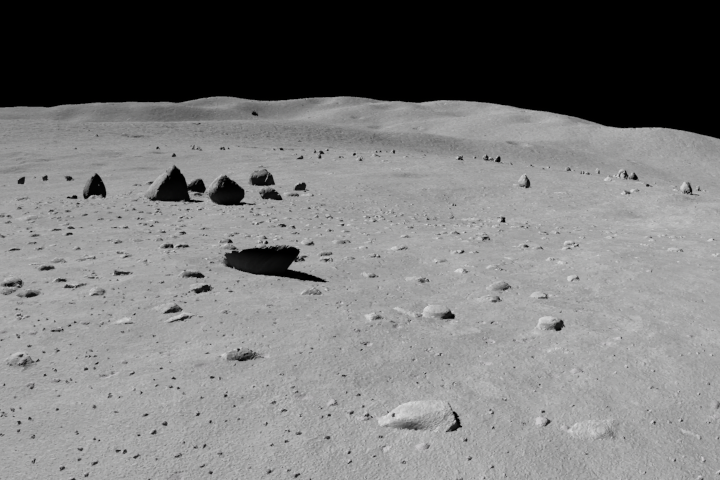
\includegraphics[width=5.5cm]{dataset_examples/Lunar/renders/render9679.png}
    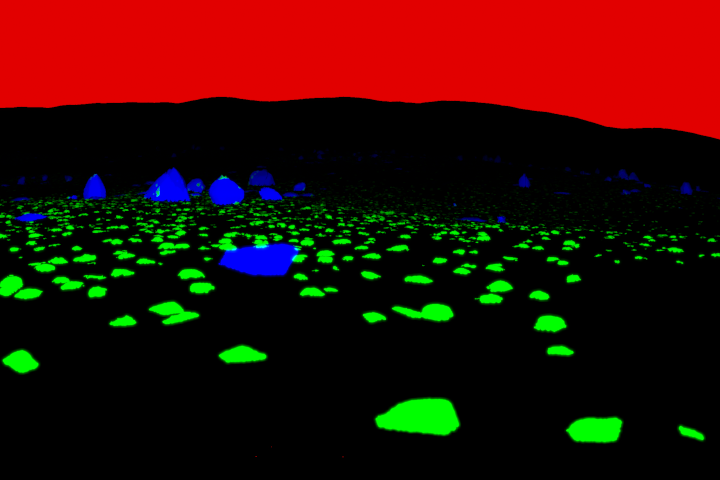
\includegraphics[width=5.5cm]{dataset_examples/Lunar/ground/ground9679.png}

    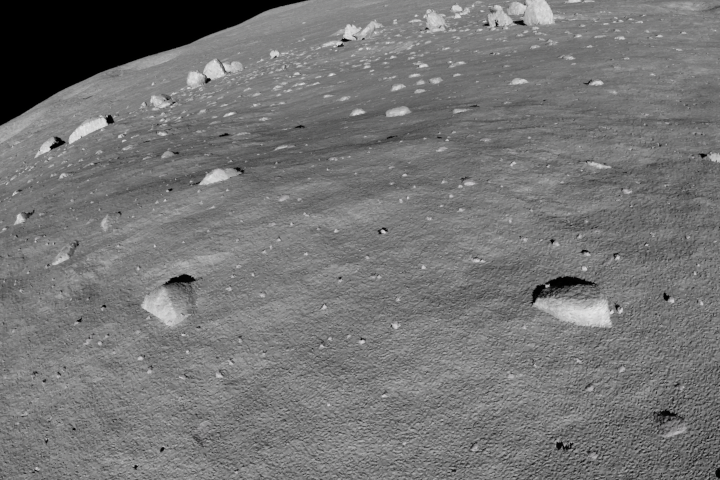
\includegraphics[width=5.5cm]{dataset_examples/Lunar/renders/render9723.png}
    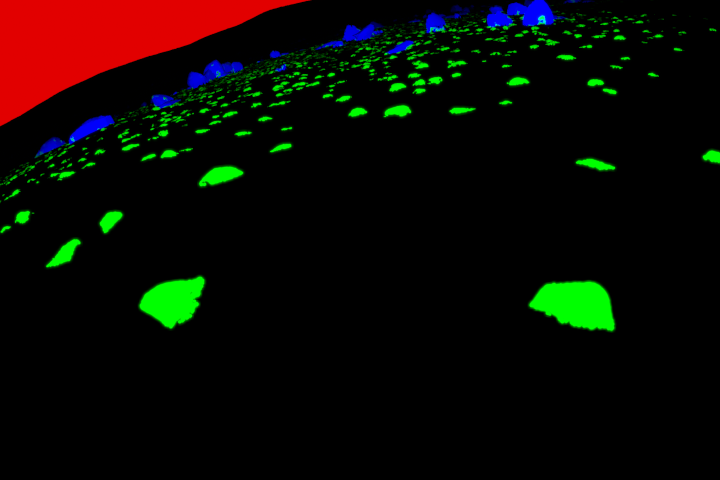
\includegraphics[width=5.5cm]{dataset_examples/Lunar/ground/ground9723.png}

    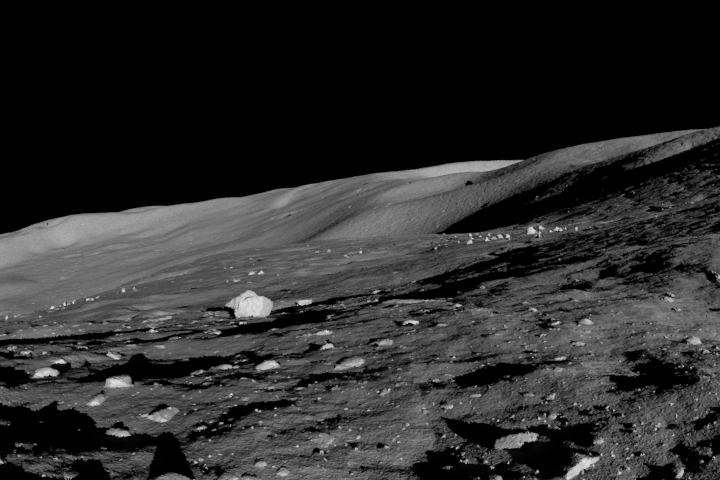
\includegraphics[width=5.5cm]{dataset_examples/Lunar/renders/render9688.png}
    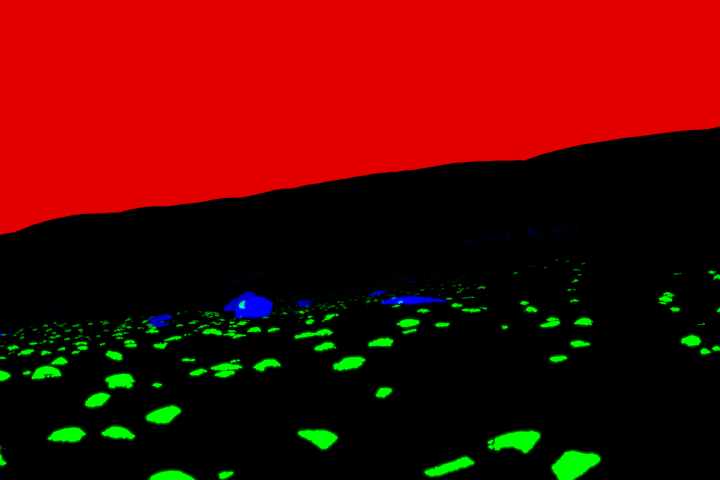
\includegraphics[width=5.5cm]{dataset_examples/Lunar/ground/ground9688.png}
    \caption{Example entries from data set with corresponding segmentation masks}
    \label{fig:data_example1}
\end{figure}

The resolution in which images are provided is $720 \times 480$ pixels. There are four segmentation classes available: large rocks (blue), smaller rocks (green), the sky (red) and everything else (black). The virtual camera capturing the renders is noise-free, and no data augmentation is performed. The position and rotation of the camera are random for each image, but the height with respect to the ground is kept low to mimic the rover's perspective. The heading and elevation of the sun are given random values for each image. Another significant property is that the colours of objects go darker with increased distance, meaning that setting the minimum intensity threshold for determining whether a certain rock should be considered is left to users. However, a threshold between 50 and 200 is recommended to avoid noise from distant rocks. Cleaned-up images of segmentation data where noise from smaller rocks is removed are also provided.

The authors also provide real lunar pictures taken by the Chang'e 3 rover equipped with two cameras to test algorithms trained on this data set. Hand-drew segmentation ground truth is also present for these pictures.

% TODO: naprawić pozycjonowanie tego
\begin{figure}[ht!]
    \centering
    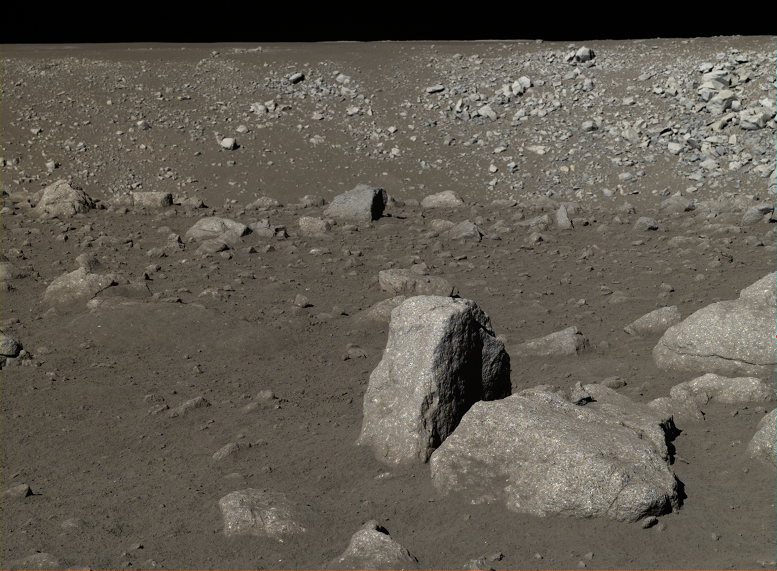
\includegraphics[width=5.5cm]{dataset_examples/Lunar/real/PCAM5.png}
    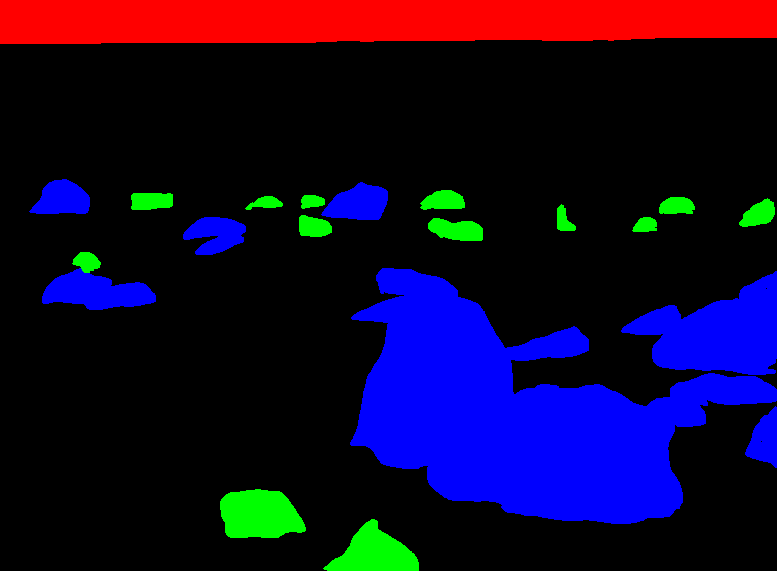
\includegraphics[width=5.5cm]{dataset_examples/Lunar/real/g_PCAM5.png}

    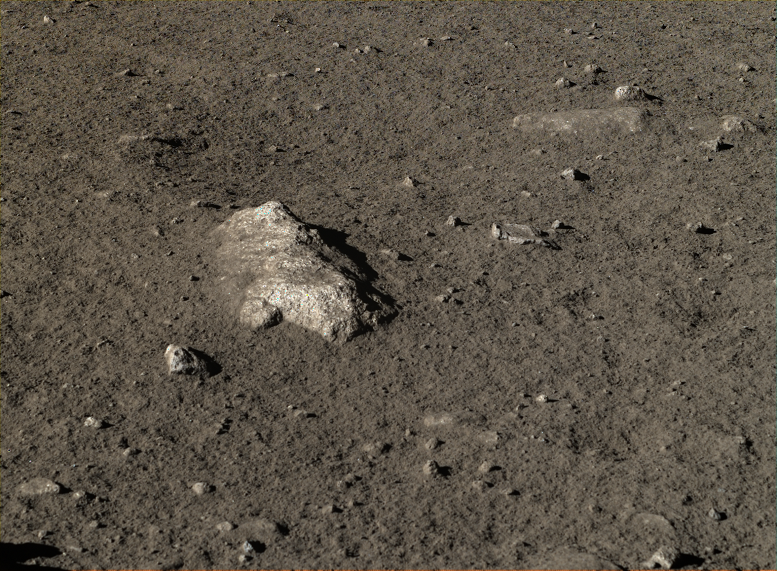
\includegraphics[width=5.5cm]{dataset_examples/Lunar/real/PCAM8.png}
    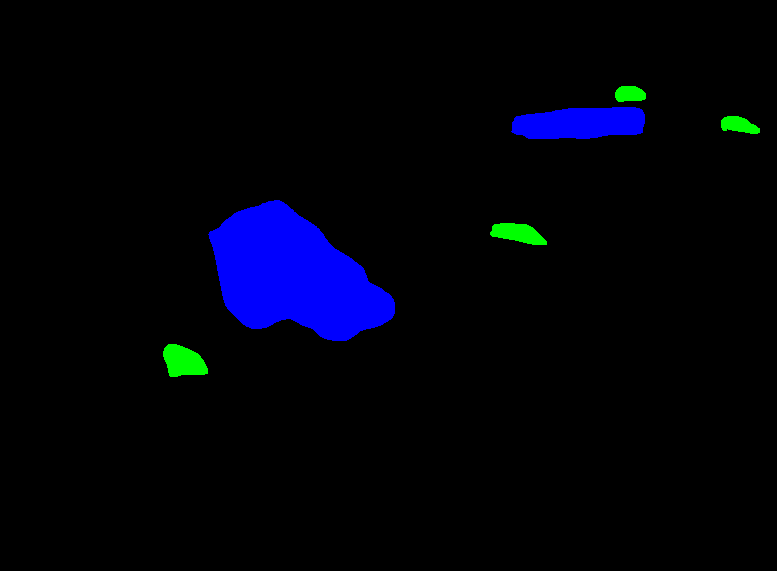
\includegraphics[width=5.5cm]{dataset_examples/Lunar/real/g_PCAM8.png}

    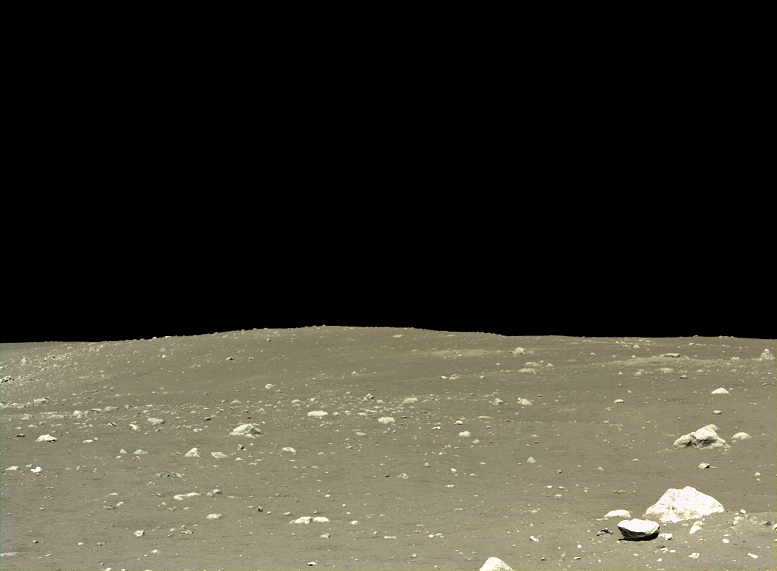
\includegraphics[width=5.5cm]{dataset_examples/Lunar/real/TCAM14.png}
    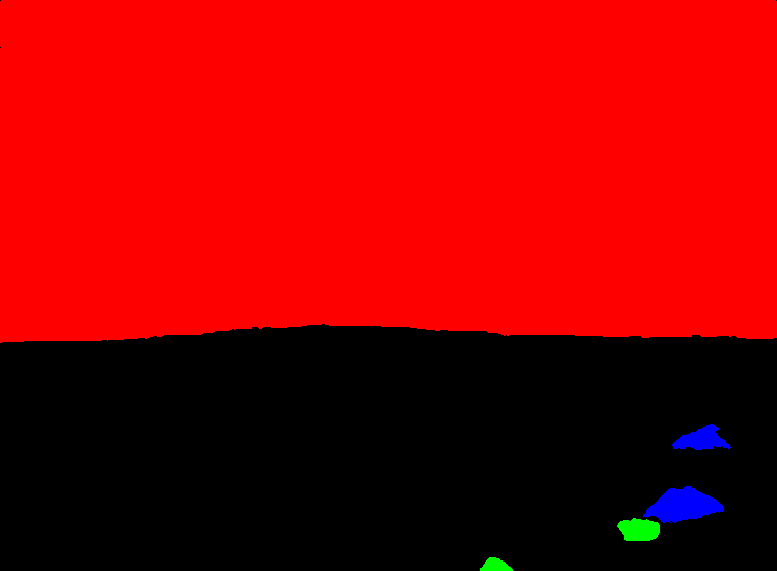
\includegraphics[width=5.5cm]{dataset_examples/Lunar/real/g_TCAM14.png}
    \caption{Example real lunar images with corresponding segmentation masks}
    \label{fig:data_real_example1}
\end{figure}

\subsection{Mars Data}
\label{sec:chapter2.1.2}
Mars Data \cite{xiao2021kernel} is a Martian rock segmentation dataset built using unlabeled images provided by NASA/JPL-Caltech. It is currently divided into two sub-datasets: Rock-A and Rock-B, with a total of 405 labelled rock images and more than 20000 rocks. Rock-A is a simpler sub-set, containing a few rocks in one image, while Rock-B is a more challenging sub-set with more abundant rocks in one scene. The authors also provide sets meant for model training and testing using data augmentation. All images are provided in $560 \times 500$ pixels resolution. Ground truth labels for this data set are only provided for binary segmentation, meaning that additional operations need to be performed in order to use this data.

\begin{figure}[!h]
    \centering
    \begin{subfigure}[b]{0.4\textwidth}
        \centering
        \caption{Rock-A}
        \includegraphics[width=3cm]{dataset_examples/Martian/Rock-A/image/964_0964ML0042700010403935E01_DXXX.jpg}
        \includegraphics[width=3cm]{dataset_examples/Martian/Rock-A/ground/964_0964ML0042700010403935E01_DXXX.png}

        \includegraphics[width=3cm]{dataset_examples/Martian/Rock-A/image/cr_116_0116MR0007330070200650E01_DXXX.jpg}
        \includegraphics[width=3cm]{dataset_examples/Martian/Rock-A/ground/cr_116_0116MR0007330070200650E01_DXXX.png}

        \includegraphics[width=3cm]{dataset_examples/Martian/Rock-A/image/cr_402_0402ML1667000000E1_DXXX.jpg}
        \includegraphics[width=3cm]{dataset_examples/Martian/Rock-A/ground/cr_402_0402ML1667000000E1_DXXX.png}


        \label{fig:rocka_martian_example}
    \end{subfigure}
    \begin{subfigure}[b]{0.4\textwidth}
        \centering
        \caption{Rock-B}
        \includegraphics[width=3cm]{dataset_examples/Martian/Rock-B/image/1580_1580ML0080490070604953E01_DXXX.jpg}
        \includegraphics[width=3cm]{dataset_examples/Martian/Rock-B/ground/1580_1580ML0080490070604953E01_DXXX.png}


        \includegraphics[width=3cm]{dataset_examples/Martian/Rock-B/image/cr_114_0114MR0006980120200632E01_DXXX.jpg}
        \includegraphics[width=3cm]{dataset_examples/Martian/Rock-B/ground/cr_114_0114MR0006980120200632E01_DXXX.png}

        \includegraphics[width=3cm]{dataset_examples/Martian/Rock-B/image/cr_714_0714MR0030410000402694E01_DXXX.jpg}
        \includegraphics[width=3cm]{dataset_examples/Martian/Rock-B/ground/cr_714_0714MR0030410000402694E01_DXXX.png}


        \label{fig:rockb_martian_example}
    \end{subfigure}
\caption{Examples Martian images with corresponding segmentation masks}
\label{fig:martian_dataset_examples}
\end{figure}

\section{Tools}
\label{sec:chapter2.2}
In this section, the most important tools which were used for data pipeline construction are presented, along with a short description. This presentation consists of modules, languages and platforms used during the execution of the project.

% Nie jestem też pewien co do tych nazw tutaj, dawać texttt czy coś podobnego?
The language used to write this project in Python. Python is a high-level, general-purpose programming language characterized by a strong emphasis on code readability and indentation, supporting multiple programming paradigms. Thanks to its simplicity and a high number of available modules, Python is widely used for data analysis and machine learning. Available modules, easiness and versatility, are the reasons why this programming language was chosen. Written code was run using the Google Collaboratory ("Colab" for short) development environment. Colab is based on the open-source project Jupyter, allowing for python code execution with the browser while providing access to computing resources such as GPUs. Highly efficient GPUs provided by Colab were crucial for this project, as the training process for deep learning algorithms requires a lot of computing resources. Another platform used for this project is the community edition of Databricks, hosting a database for storing experiment results using the open-source MlFlow platform.

The most important Python modules used in the project are:
\begin{itemize}
    \item \texttt{Pandas} is an open-source data analysis and manipulation tool. It offers data structures for fast and flexible tabular data manipulation and tools for reading and writing data between memory and files.

    \item \texttt{NumPy} is an open-source module providing support for large, multi-dimensional arrays and matrices, along with many high-level mathematical functions to operate on these matrices. This module is used in nearly every scientific domain. This project came useful in manipulating images for this work.

    \item \texttt{Matplotlib} is a comprehensive library for creating static, animated and interactive visualizations in Python. In this work, \texttt{matplotlib} was used for creating plots visualizing the obtained results.

    \item \texttt{OpenCV} is a library of programming functions mainly aimed at real-time computer vision. In this project, it is mostly used for manipulating images.

    \item \texttt{TensorFlow} is an open-source library for machine learning and artificial intelligence, available in many programming languages, including Python. It can be used across various tasks but focuses mostly on training and inference of deep neural networks.

    \item \texttt{Keras} is an open-source library that acts as an interface for \texttt{TensorFlow}, designed to enable fast experimentation with deep neural networks.

    \item \texttt{Segmentation models} is a python library with neural networks for image segmentation based on \texttt{Keras} and \texttt{TensorFlow}. This library provides a high-level API with multiple model architectures and backbones.

    \item \texttt{MLflow} is a platform for machine learning development, offering a set of lightweight APIs that can be used with any existing machine learning library. The component mostly used in this project is MLflow Tracking - an API to log models, parameters and results.
\end{itemize}

\section{Image Segmentation}
\label{sec:chapter2.3}
The problem of image segmentation has been inseparable from the field of computer vision since the early days, as it is an essential component of visual understanding systems. It involves partitioning images into multiple images and segments and has multiple applications, including medical image analysis, augmented reality and autonomous vehicles. This section is an overview of what methods can be applied to the problem of segmentation. % Tutaj też coś dalej na temat tego jakie są wykorzystywane i po co taki rozdział jest

Image segmentation can be formulated as a problem of assigning every pixel of an input image to a semantic label semantic segmentation) or partitioning of individual objects (instance segmentation). It is generally more demanding than image classification, which predicts a single label for the entire image. Different image segmentation algorithms have been proposed in the literature, with the earliest methods being thresholding \cite{otsu1979threshold}, region-growing \cite{nock2004statistical}, k-mean clustering \cite{dhanachandra2015image} to more sophisticated methods such as active contours \cite{kass1988snakes}, conditional and Markov random fields \cite{plath2009multi}, and sparsity-based methods \cite{starck2005image}. A paradigm shift in the field has been caused by deep learning models, raising a new generation of segmentation models with unprecedented performance improvements, achieving the highest accuracy rates on popular benchmarks.

%Tutaj ogólnie spoko by było dodać jakieś wizualizacje - zapytać czy w końcu można się odnosić do rysunków z innych prac czy nie
Most image segmentation algorithms are built using the Convolutional Neural Networks (CNNs) architecture, widely used for computer vision problems. CNNs architectures usually consist of three types of layers: convolutional layers, where a kernel of weights is convoluted for feature extraction; pooling layers which reduce the spatial resolution by replacing small neighbourhoods in a feature mas with statistical information about those neighbourhoods and nonlinear layers; which apply an activation function to feature maps, enabling the network to model nonlinear functions. The layers are stacked to form multiresolution pyramids, where the high-level layers learn features from increasingly wider receptive fields. The main advantage over fully-connected neural networks is that all the receptive fields in a layer share weights, resulting in a significantly smaller number of parameters.


Other important architectures for image segmentation are Encoder-Decoder and Auto-Encoder models. Encoder-decoder models learn to represent input data points to output using a two-stage network. The encoder part compresses the input $x$ into a latent space representation $z$, performing an encoding function $z = g(x)$. The decoder part predicts the output $y$ on the basis of latent representation $z$, performing a decoding operation $y = f(z)$. The latent space represents the semantic information of the input useful in predicting the output. Such models are popular for sequence-to-sequence modelling in Natural Language Processing and image-to-image translation in applications where the output is an improved version of the input image or a segmentation map. Autoencoders are a special case of encoder-decoder models where the input and output are the same.

Some of the deep learning architectures used for semantic segmentation are: % Tutaj może być coś więcej ale na ten moment nie mam pomysłu
\begin{itemize}
    % Tutaj może też by się dało coś jeszcze napisać
    % dodatkowo możnaby podkreślić nieco nazwę tych architektur ale nie mam pomysłu jak na ten moment
    \item \textbf{Fully Convolutional Models (FCNs)}, proposed by Long \textit{et al.} \cite{long2015fully}, are made out of only convolutional layers. Enabling the output segmentation maps to be the same size as the input image is possible using skip connections in which feature maps are up-sampled from the final layer and fused with feature maps from previous layers. FCNs can achieve state-of-the-art performance but are computationally too expensive for real-time inference and is not easily generalizable to 3D images.

    \item \textbf{Encoder-decoder} architecture, used by some of the most popular deep learning-based algorithms. Semantic segmentation based on deconvolution was introduced by Noh \textit{et al.} in \cite{noh2015learning}, where a model is made up of two parts, an encoder using convolutional layers adopted from the VGG network and a deconvolutional network that generates class predictions for every pixel of the input image. The limitation of this architecture is that the fine-grained image information is lost during the encoding process. This issue was addressed in later models, which maintain the resolution by connecting the convolution streams in parallel and repeatedly exchanging information across resolutions.

    \item \textbf{U-Net} architecture, proposed in 2015 by Ronneberger \textit{et al.} \cite{ronneberger2015u}, follows similar architectural principles as encoder-decoder architecture, where the encoder path captures the context and the symmetrical decoder part enables for precise location of objects in the input image. To combat the information loss during the decoding process, U-Net architecture is extended using skip connections from the encoder block layers to their symmetric counterparts in the decoder block. This procedure enables detail preservation and consideration of different abstraction levels. This architecture was initially created for medical image segmentation but was proven to excel in different domains. Additionally, this architecture can be generalized for use with 3D images.

    \item \textbf{Multiscale based} architecture employs multiscale analysis. One of the most notable models using this architecture is the Feature Pyramid Network (FPN) proposed by Lin \textit{et al.} \cite{lin2017feature}, which was initially developed for object detection, but is also applicable for image segmentation. In this architecture, a feature pyramid is constructed using an inherent multiscale pyramidal hierarchy of deep CNNs. The FPN is composed of bottom-up and top-down pathways and lateral connections in order to merge low and high-resolution features.

    \item \textbf{Pyramid network based} architecture was developed by Zhao \textit{et atl.} \cite{zhao2017pyramid} better to learn the global context representation of a scene. A residual network is used as a feature extractor to extract multiple patterns from the input image. These feature maps are then passed into a pyramid pooling module to distinguish different scales of patterns. The outputs of the pyramid levels are then up-sampled and connected with the initial feature maps to capture the global and local information. To generate pixel-wise predictions, a convolutional layer is used.

% Chyba wystarczy do tej sekcji ale można by tu jeszcze coś napisać
\end{itemize}


These are not all deep neural network architectures used for semantic segmentation. However, the listed architectures are already widely used and have proven to produce high-quality results. They will also be used in this project for rock segmentation.

\section{Edge deep learning}
\label{sec:chapter2.4}

The state-of-the-art deep learning algorithms have proven to be capable of solving complex problems and are now used in a wide range of services and applications. Nonetheless, these algorithms require the availability of high-performance hardware with a large amount of storage\cite{najafabadi2015deep}. The preferred way for running machine learning models has been \emph{cloud computing}, realised using data centres with huge amounts of space and computational resources.

However, with the increasing number of devices with limited resources using machine learning algorithms to make predictions, the available bandwidth has become a bottleneck. Additionally, more latency-constrained devices have begun to use deep-learning models, such as autonomous vehicles \cite{grigorescu2020survey}. The limitations of limited resource devices lead to the creation of a new paradigm called \emph{edge computing}, bringing the calculation as locally as possible. As edge devices have limited computational resources, machine learning algorithms must be especially suited for constrained execution. It is also possible because the inference phase requires significantly fewer resources than the training phase. The paradigm of using highly efficient and accurate deep learning methods in low-power hardware-constrained devices can also be applied to challenging space exploration problems. % Tutaj jeszcze nie jestem pewine tego zdania, może się albo zmienić albo coś jeszcze można dopisać

Usually, the design of deep learning models is oriented towards achieving the best accuracy. However, when other metrics are considered, such as performance, cost or energy, more accurate models are not necessarily better \cite{vestias2020moving}. When considering the number of parameters, a small decrease in accuracy is acceptable in exchange for a significant reduction. Fewer network parameters mean less memory is used, and the inference time is reduced. Apart from designing edge-oriented architectures, several optimization techniques exist for reducing the number of parameters of already existing models in exchange for a minor reduction in accuracy. The two main classes of optimizations are data quantization and data reduction.

Data quantization methods reduce the complexity of operations and the number of bits representing parameters. Typically, model weights are stored inside \texttt{float32} variables. The hardware implementation is more complex for floating-point arithmetics than for fixed-point or integer, as the amount of bits representing data determines the complexity of operations. The post-quantization technique reduces the variables storing weights from 32 bits to 16 or 8 bits, obtaining models 2 to 4 times smaller. The authors of \cite{gysel2016hardware} show that using 8 bit variables for parameters has a neglectable accuracy impact. Representations of models with 16 or 8 bits also considerably reduce the complexity of operations.

Another optimization method is data reduction, decreasing the number of parameters to reduce memory storage, memory bandwidth requirements and the number of computations. The first data reduction approach has been proposed by Han \textit{et al.} in \cite{han2015deep}, which consists of pruning and compression with Huffman coding. Pruning is the process of removing network connections, which introduces sparsity into the matrix of weights. Although it reduces the number of connections, it also results in irregular access to on-chip memory. In models based on convolutional layers, it is possible to use the Winograd filtering technique \cite{winograd1980arithmetic} to calculate convolutions \cite{lavin2016fast}, reducing the number of multiplications.

% TODO: tutaj może jeszcze jakieś podsumowanie tej sekcji

%Tak w sumie to średnio jestem przekonany czy taka sekcja powinna tutaj być
\section{Data pipeline}
Considering all of the techniques mentioned above, combining deep learning algorithms with optimization is possible to obtain an efficient and accurate algorithm for rock segmentation. The steps of this process are as follows:
\begin{enumerate}
    \item loading the data
    \item splitting the data into train, validation and test sets
    \item training the model o choice
    \item measuring the performance of the trained model
    \item adjusting the model accordingly to the obtained metrics
\end{enumerate}

\section{Model evaluation metrics}
%Taka sekcja też musi być, nie wiem tylko czy tutaj czy w następnym rozdziale

% może tutaj jakieś podsumowanie całego rozdziału
\chapter{Obtained results}
\label{sec:chapter3}
%Tutaj jeszcze spoko będzie parę słów wprowadzenia

\section{Project overview}
\label{sec:chapter3.1}
The Artificial Lunar Landscape data set, along with the render images, also provides two types of ground truth sets, one with every rock on the scene marked and the other cleaned by authors. Unfortunately, the cleaned set does not cover all rocks important to the scene. Therefore, manual cleaning has to be performed while reading the ground truth images. As the authors suggest a colour threshold between 50 to 200, the threshold has been chosen to be 100 in order to preserve all important information on the scene and filter out noise from distant rocks. The RGB values from ground images are then clipped to correspond to numerical labels.  %tutaj może jakiś przykład jak to wygląda będzie git


In order to fit within the memory of the graphical processing unit, the input images were rescaled to a resolution of $320 \times 320$ pixels and the batch size was set to 16. The whole input set was divided so that the test and validation sets contained 1000 images, and the rest was put into the training set. To further enhance the models' ability to generalize, data augmentation using the \texttt{imgaug} module has been introduced on training and validation sets, consisting of vertical and horizontal flipping in 50\% of inputs, cropping 10\% of image and changing linear contrast.

% Zdaję sobię sprawę że ten akapit może być trochę niejasny i zagmatwany
The algorithms are created using the \texttt{segmentation models} library, allowing for combining all available encoders and architectures. All encoders available in this library are also pre-trained on the ImageNet data set for faster convergence. The \texttt{segmentation models} library is used with the \texttt{TensorFlow} library as a back end. The parameters of the network were automatically logged during training, using \texttt{MLflow} library. During training, the \texttt{Adam} optimizer is used along with dice loss. A callback is set using the \texttt{Keras} library for early stopping when the validation loss stops improving over five epochs; then, the best weights are restored.
% To chyba tyle, potem opisać jaka architekura i jakie enkodery zostały wybrane na początek i dlaczego, ale to może być też w następnej sekcji

\section{Initial results}
\label{sec:chapter3.2}

% % TODO
% \chapter{Requirements and tools}

% \begin{itemize}
% \item functional and nonfunctional requirements
% \item use cases (UML diagrams)
% \item description of tools
% \item methodology of design and implementation
% \end{itemize}

% % TODO
% \chapter{External specification}
% \begin{itemize}
% \item hardware and software requirements
% \item installation procedure
% \item activation procedure
% \item types of users
% \item user manual
% \item system administration
% \item security issues
% \item example of usage
% \item working scenarios (with screenshots or output files)
% \end{itemize}


%%%%%%%%%%%%%%%%%%%%%


%%%%%%%%%%%%%%%%%%%%
%% SUBFIGURES
%
%\begin{figure}
%\centering
%\begin{subfigure}{0.4\textwidth}
%    
\includegraphics[width=\textwidth]{./politechnika_sl_logo_bw_pion_en.pdf}
%    \caption{Upper left figure.}
%    \label{fig:upper-left}
%\end{subfigure}
%\hfill
%\begin{subfigure}{0.4\textwidth}
%    
\includegraphics[width=\textwidth]{./politechnika_sl_logo_bw_pion_en.pdf}
%    \caption{Upper right figure.}
%    \label{fig:upper-right}
%\end{subfigure}
%
%\begin{subfigure}{0.4\textwidth}
%    
\includegraphics[width=\textwidth]{./politechnika_sl_logo_bw_pion_en.pdf}
%    \caption{Lower left figure.}
%    \label{fig:lower-left}
%\end{subfigure}
%\hfill
%\begin{subfigure}{0.4\textwidth}
%    
\includegraphics[width=\textwidth]{./politechnika_sl_logo_bw_pion_en.pdf}
%    \caption{Lower right figure.}
%    \label{fig:lower-right}
%\end{subfigure}
%
%\caption{Common caption for all subfigures.}
%\label{fig:subfigures}
%\end{figure}
%Fig. \ref{fig:subfigures} presents very important information, eg. Fig. \ref{fig:upper-right} is an upper right subfigure.
%%%%%%%%%%%%%%%%%%%%%


% % TODO
% \chapter{Internal specification}

% \begin{itemize}
% \item concept of the system
% \item system architecture
% \item description of data structures (and data bases)
% \item components, modules, libraries, resume of important classes (if used)
% \item resume of important algorithms (if used)
% \item details of implementation of selected parts
% \item applied design patterns
% \item UML diagrams
% \end{itemize}



% % % % % % % % % % % % % % % % % % % % % % % % % % % % % % % % % % %
% To use the minted packages uncomment the package import in        %
% file config/settings.tex :  \usepackage{minted}                   %
% and compile with the shell escape                                 %
% pdflatex -shell-escape main                                       %
% % % % % % % % % % % % % % % % % % % % % % % % % % % % % % % % % % %


% Use special environments for inline code, eg  \lstinline|int a;| (package \texttt{listings})% or  \mintinline{C++}|int a;| (package \texttt{minted})
% . Longer parts of code put in the figure environment, eg. code in Fig. \ref{fig:pseudocode:listings}% and Fig. \ref{fig:pseudocode:minted}
% . Very long listings–move to an appendix.


% \clearpage
% \begin{figure}
% \centering
% \begin{lstlisting}
% class test : public basic
% {
%     public:
%       test (int a);
%       friend std::ostream operator<<(std::ostream & s,
%                                      const test & t);
%     protected:
%       int _a;

% };
% \end{lstlisting}
% \caption{Pseudocode in \texttt{listings}.}
% \label{fig:pseudocode:listings}
% \end{figure}

% %\begin{figure}
% %\centering
% %\begin{minted}[linenos,frame=lines]{c++}
% %class test : public basic
% %{
% %    public:
% %      test (int a);
% %      friend std::ostream operator<<(std::ostream & s,
% %                                     const test & t);
% %    protected:
% %      int _a;
% %
% %};
% %\end{minted}
% %\caption{Pseudocode in \texttt{minted}.}
% %\label{fig:pseudocode:minted}
% %\end{figure}




% % TODO
% \chapter{Verification and validation}
% \begin{itemize}
% \item testing paradigm (eg V model)
% \item test cases, testing scope (full / partial)
% \item detected and fixed bugs
% \item results of experiments (optional)
% \end{itemize}


% \begin{table}
% \centering
% \caption{A caption of a table is \textbf{above} it.}
% \label{id:tab:wyniki}
% \begin{tabular}{rrrrrrrr}
% \toprule
% 	         &                                     \multicolumn{7}{c}{method}                                      \\
% 	         \cmidrule{2-8}
% 	         &         &         &        \multicolumn{3}{c}{alg. 3}        & \multicolumn{2}{c}{alg. 4, $\gamma = 2$} \\
% 	         \cmidrule(r){4-6}\cmidrule(r){7-8}
% 	$\zeta$ &     alg. 1 &   alg. 2 & $\alpha= 1.5$ & $\alpha= 2$ & $\alpha= 3$ &   $\beta = 0.1$  &   $\beta = -0.1$ \\
% \midrule
% 	       0 &  8.3250 & 1.45305 &       7.5791 &    14.8517 &    20.0028 & 1.16396 &                       1.1365 \\
% 	       5 &  0.6111 & 2.27126 &       6.9952 &    13.8560 &    18.6064 & 1.18659 &                       1.1630 \\
% 	      10 & 11.6126 & 2.69218 &       6.2520 &    12.5202 &    16.8278 & 1.23180 &                       1.2045 \\
% 	      15 &  0.5665 & 2.95046 &       5.7753 &    11.4588 &    15.4837 & 1.25131 &                       1.2614 \\
% 	      20 & 15.8728 & 3.07225 &       5.3071 &    10.3935 &    13.8738 & 1.25307 &                       1.2217 \\
% 	      25 &  0.9791 & 3.19034 &       5.4575 &     9.9533 &    13.0721 & 1.27104 &                       1.2640 \\
% 	      30 &  2.0228 & 3.27474 &       5.7461 &     9.7164 &    12.2637 & 1.33404 &                       1.3209 \\
% 	      35 & 13.4210 & 3.36086 &       6.6735 &    10.0442 &    12.0270 & 1.35385 &                       1.3059 \\
% 	      40 & 13.2226 & 3.36420 &       7.7248 &    10.4495 &    12.0379 & 1.34919 &                       1.2768 \\
% 	      45 & 12.8445 & 3.47436 &       8.5539 &    10.8552 &    12.2773 & 1.42303 &                       1.4362 \\
% 	      50 & 12.9245 & 3.58228 &       9.2702 &    11.2183 &    12.3990 & 1.40922 &                       1.3724 \\
% \bottomrule
% \end{tabular}
% \end{table}



% % TODO
% \chapter{Conclusions}
% \begin{itemize}
% \item achieved results with regard to objectives of the thesis and requirements
% \item path of further development (eg functional extension …)
% \item encountered difficulties and problems
% \end{itemize}



\backmatter

%\bibliographystyle{plain}  % bibtex
%\bibliography{biblio} % bibtex
\printbibliography           % biblatex
\addcontentsline{toc}{chapter}{References}

\begin{appendices}

% TODO

\chapter{Index of abbreviations and symbols}

\begin{itemize}
\item[DNA] deoxyribonucleic acid
\item[MVC] model--view--controller
\item[$N$] cardinality of data set
\item[$\mu$] membership function of a fuzzy set
\item[$\mathbb{E}$] set of edges of a graph
\item[$\mathcal{L}$] Laplace transformation
\end{itemize}


% TODO
\chapter{Listings}

(Put long listings here.)

\begin{lstlisting}
if (_nClusters < 1)
	throw std::string ("unknown number of clusters");
if (_nIterations < 1 and _epsilon < 0)
	throw std::string ("You should set a maximal number of iteration or minimal difference -- epsilon.");
if (_nIterations > 0 and _epsilon > 0)
	throw std::string ("Both number of iterations and minimal epsilon set -- you should set either number of iterations or minimal epsilon.");
\end{lstlisting}


% % % % % % % % % % % % % % % % % % % % % % % % % % % % % % % % % % %
% To use the minted packages uncomment the package import in        %
% file config/settings.tex :  \usepackage{minted}                   %
% and compile with the shell escape                                 %
% pdflatex -shell-escape main                                       %
% % % % % % % % % % % % % % % % % % % % % % % % % % % % % % % % % % %

%\begin{minted}[linenos,breaklines,frame=lines]{c++}
%if (_nClusters < 1)
%	throw std::string ("unknown number of clusters");
%if (_nIterations < 1 and _epsilon < 0)
%	throw std::string ("You should set a maximal number of iteration or minimal difference -- epsilon.");
%if (_nIterations > 0 and _epsilon > 0)
%	throw std::string ("Both number of iterations and minimal epsilon set -- you should set either number of iterations or minimal epsilon.");
%\end{minted}

% TODO
\chapter{List of additional files in~electronic submission (if applicable)}


Additional files uploaded to the system include:
\begin{itemize}
\item source code of the application,
\item test data,
\item a video file showing how software or hardware developed for thesis is used,
\item etc.
\end{itemize}

\listoffigures
\addcontentsline{toc}{chapter}{List of figures}
\listoftables
\addcontentsline{toc}{chapter}{List of tables}

\end{appendices}

\end{document}


%% Finis coronat opus.

